\documentclass[tikz,border=2pt]{standalone}
\usepackage{unicode-math}
\setmainfont[
  Path=publication/fonts/,
  UprightFont=source-serif-4-latin-400-normal.ttf,
  ItalicFont=source-serif-4-latin-400-italic.ttf,
  BoldFont=source-serif-4-latin-600-normal.ttf,
  BoldItalicFont=source-serif-4-latin-600-italic.ttf
]{Source Serif 4}
\setmathfont[Path=/System/Library/Fonts/Supplemental/]{STIXTwoMath.otf}
\usepackage{tikz}
\usetikzlibrary{arrows.meta,backgrounds,calc,decorations.pathreplacing,fit,matrix,positioning}
\definecolor{BookInk}{HTML}{18232D}
\definecolor{BookBlue}{HTML}{315F78}
\definecolor{BookRed}{HTML}{98452F}
\definecolor{BookGreen}{HTML}{3F6659}
\definecolor{BookMuted}{HTML}{66727A}
\definecolor{BookRule}{HTML}{AEB7BC}
\tikzset{
  book/node/.style={
    draw=BookInk, line width=.55pt, fill=white,
    minimum height=9mm, inner xsep=5pt, inner ysep=4pt,
    font=\footnotesize, align=center
  },
  book/primary/.style={book/node, draw=BookBlue},
  book/decision/.style={book/node, draw=BookRed},
  book/verified/.style={book/node, draw=BookGreen},
  book/arrow/.style={
    -{Stealth[length=2mm,width=1.35mm]}, line width=.55pt, draw=BookInk
  },
  book/quietarrow/.style={
    -{Stealth[length=2mm,width=1.35mm]}, line width=.45pt, draw=BookRule
  },
  book/feedback/.style={
    -{Stealth[length=2mm,width=1.35mm]}, line width=.5pt,
    draw=BookRed, dashed
  },
  book/note/.style={font=\scriptsize, text=BookMuted, align=center}
}

\begin{document}
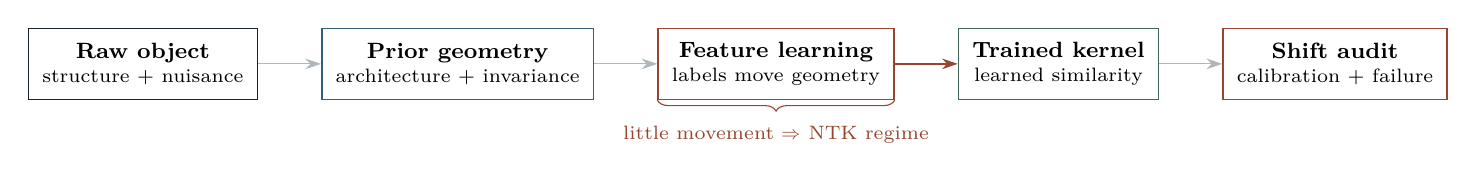
\begin{tikzpicture}[node distance=8mm]
  \node[book/node] (raw) {\textbf{Raw object}\\[-1pt]\scriptsize structure + nuisance};
  \node[book/primary,right=of raw] (prior) {\textbf{Prior geometry}\\[-1pt]\scriptsize architecture + invariance};
  \node[book/decision,right=of prior] (learn) {\textbf{Feature learning}\\[-1pt]\scriptsize labels move geometry};
  \node[book/verified,right=of learn] (kernel) {\textbf{Trained kernel}\\[-1pt]\scriptsize learned similarity};
  \node[book/decision,right=of kernel] (audit) {\textbf{Shift audit}\\[-1pt]\scriptsize calibration + failure};
  \draw[book/quietarrow] (raw.east)--(prior.west);
  \draw[book/quietarrow] (prior.east)--(learn.west);
  \draw[book/arrow,draw=BookRed] (learn.east)--(kernel.west);
  \draw[book/quietarrow] (kernel.east)--(audit.west);
  \draw[decorate,decoration={brace,amplitude=4pt,mirror},BookRed]
    (learn.south west) -- (learn.south east)
    node[midway,below=6pt,book/note,text=BookRed]
      {little movement $\Rightarrow$ NTK regime};
\end{tikzpicture}
\end{document}
